\documentclass[12pt, a4paper]{article}

% Pengaturan bahasa dan font
\usepackage[utf8]{inputenc}
\usepackage[indonesian]{babel}
\usepackage{mathptmx} % Font Times New Roman
\usepackage[T1]{fontenc}

% Pengaturan margin
\usepackage[top=3cm, bottom=3cm, left=3cm, right=3cm]{geometry}

% Pengaturan paragraf dan spasi
\usepackage{setspace}
\onehalfspacing % Spasi 1.5 baris seperti standar Word
\usepackage{indentfirst} % Paragraf pertama menjorok ke dalam

% Gambar
\usepackage{graphicx}

% Pengaturan judul Bab agar rapi dan tidak terlalu besar
\usepackage{titlesec}
\titleformat{\section}{\normalfont\large\bfseries\centering}{BAB \Roman{section}}{1em}{}
\titleformat{\subsection}{\normalfont\normalsize\bfseries}{\thesubsection}{1em}{}

% Pengaturan Daftar Isi agar menggunakan titik-titik (dot leaders)
\usepackage{tocloft}
\renewcommand{\cftsecleader}{\cftdotfill{\cftdotsep}}

\addto\captionsindonesian{%
    \renewcommand{\contentsname}{\centerline{\Large\bfseries DAFTAR ISI}}%
}

\begin{document}

% ================= COVER =================
\begin{titlepage}
    \centering
    \vspace*{2cm}
    
    {\Large \textbf{PROPOSAL BISNIS IoT}}\\[0.5cm]
    {\Large \textbf{Smart Server Room Monitor (SSRM)}}\\[0.5cm]
    {\Large \textbf{NusaMonitor Tech}}\\[1cm]
    
    % Pastikan file images.png ada di folder yang sama, atau hapus baris ini jika tidak menggunakan gambar
    
\includegraphics[width=10cm]{images.png}\\[1cm]
    
    {\normalsize \textbf{Disusun Oleh Kelompok 4:}}\\[0.5cm]
    
    \begin{tabular}{ll}
        1. & Wisam Yassar Mahardika \\
        2. & Devant Fadhillah \\
        3. & Sandika Eka Permadi\\
        4. & Rafli Saeful Rukmana\\
        5. & Aliif Abdu Mukti Al-Ghifari \\
    \end{tabular} \\[0.4cm]
    
    \vfill
    
    {\normalsize \textbf{SMK Plus Pratama Adi}}\\
    {\normalsize \textbf{TAHUN 2026}}
\end{titlepage}

\newpage

% ================= KATA PENGANTAR =================
\section*{KATA PENGANTAR}
\addcontentsline{toc}{section}{KATA PENGANTAR}

Puji syukur kami panjatkan ke hadirat Tuhan Yang Maha Esa atas rahmat dan karunia-Nya sehingga proposal bisnis \textit{Internet of Things} (IoT) yang berjudul ``Smart Server Room Monitor'' ini dapat diselesaikan dengan baik.

Proposal ini disusun untuk memenuhi tugas mata pelajaran Kreativitas dan Inovasi Kewirausahaan (KIK) sekaligus menjabarkan rencana bisnis nyata terkait produk pemantauan suhu dan keamanan fisik untuk ruang server berskala kecil hingga menengah. Kami menyadari bahwa infrastruktur jaringan komputer (TKJ) membutuhkan lingkungan yang stabil, sehingga produk ini dirancang sebagai solusi yang praktis dan dapat diaplikasikan secara nyata.

Kami mengucapkan terima kasih kepada Bapak/Ibu Guru pembimbing dan semua pihak yang telah memberikan dukungan dalam penyusunan proposal ini. Kami berharap proposal ini tidak hanya sekadar menjadi tugas akademis, tetapi juga dapat menjadi pijakan awal dalam melatih keterampilan kewirausahaan kami di bidang teknologi.

\vspace{2cm}
\begin{flushright}
Penyusun, \\
\vspace{1.5cm}
Tim NusaMonitor Tech
\end{flushright}

\newpage

% ================= DAFTAR ISI =================
\tableofcontents
\newpage

% ================= BAB I =================
\section{PENDAHULUAN}

\subsection{Latar Belakang}
Peralatan jaringan dan komputer seperti \textit{server}, \textit{router}, dan \textit{switch} membutuhkan suhu ruangan yang terjaga untuk dapat beroperasi dengan optimal. Panas berlebih (\textit{overheating}) sering kali menjadi penyebab utama kerusakan perangkat keras yang berakibat pada berhentinya layanan jaringan (\textit{downtime}). Sayangnya, sistem pemantauan ruang server berstandar industri biasanya membutuhkan biaya yang sangat mahal, sehingga kurang terjangkau bagi sekolah atau instansi tingkat menengah. Hal ini membuka peluang bagi kami untuk membuat produk teknologi tepat guna.

\subsection{Rumusan Masalah}
Berdasarkan latar belakang tersebut, rumusan masalah dalam proposal bisnis ini adalah bagaimana merancang dan membuat sistem pemantauan suhu, kelembapan, dan alarm ruang server secara \textit{real-time} yang harganya terjangkau bagi instansi menengah ke bawah tanpa mengorbankan fungsi utamanya.

\subsection{Tujuan}
Tujuan dari bisnis ini adalah memproduksi dan memasarkan ``Smart Server Room Monitor''. Sistem IoT ini bertujuan memberikan kemudahan pemantauan jarak jauh yang mampu memberikan peringatan dini kepada administrator jaringan, sekaligus menjadi sarana praktik pembuatan produk kreatif bagi kelompok kami.

\subsection{Manfaat}
Bagi konsumen, produk ini bermanfaat untuk mencegah kerusakan perangkat keras IT dan menghemat biaya perbaikan. Bagi kami selaku siswa, proyek ini bermanfaat untuk mengasah keterampilan teknis jurusan TKJ sekaligus melatih kemampuan berwirausaha dalam menjual produk hasil karya sendiri.

% ================= BAB II =================
\section{PROFIL USAHA}

\subsection{Nama Usaha}
Nama usaha kami adalah \textbf{NusaMonitor Tech}. Nama ini mencerminkan identitas kami sebagai pembuat solusi pemantauan berbasis teknologi dari karya anak bangsa yang dapat diandalkan.

\subsection{Logo}
Logo usaha kami menggunakan elemen visual yang dapat dilihat pada gambar sampul dokumen ini. 

\subsection{Makna Logo}
Elemen dalam logo tersebut merepresentasikan konektivitas antapperangkat (simbol nirkabel/node), perlindungan aset IT (simbol perisai/gembok), serta integrasi pelaporan data melalui teknologi komputasi awan (\textit{cloud}). Warna yang digunakan melambangkan kepercayaan dan inovasi masa depan.

\subsection{Visi dan Misi}
\textbf{Visi} kami adalah menjadi penyedia solusi manajemen infrastruktur IT yang paling terjangkau dan inovatif bagi institusi pendidikan dan UMKM di Indonesia. \\
\textbf{Misi} kami meliputi:
\begin{enumerate}
    \item Menciptakan produk IoT dengan konsep \textit{plug-and-play} yang mudah diinstalasi.
    \item Memberikan layanan purnajual dan garansi yang responsif bagi setiap klien.
    \item Mengedukasi segmen pasar menengah mengenai pentingnya tindakan preventif dalam perlindungan aset IT.
\end{enumerate}

\subsection{Target Pasar}
Target segmen pasar utama produk kami adalah:
\begin{itemize}
    \item Sekolah menengah dan kejuruan yang memiliki fasilitas laboratorium komputer mandiri.
    \item Perusahaan skala UMKM menengah yang memiliki rak jaringan (\textit{network rack}) internal.
    \item Instansi pemerintahan desa/daerah yang memiliki ruang server dengan anggaran IT yang terbatas.
\end{itemize}

% ================= BAB III =================
\section{PRODUK/JASA}

\subsection{Deskripsi}
Smart Server Room Monitor adalah inovasi sistem pemantauan lingkungan IT terpusat. Sistem ini memanfaatkan \textit{microcontroller} cerdas ESP32 D1 R32 sebagai unit pemroses utama dan pembaca sensor (suhu dan kelembapan) yang diletakkan langsung di dalam rak server, dilengkapi dengan layar OLED dan alarm peringatan (\textit{buzzer}) terintegrasi.

\subsection{Keunggulan}
Keunggulan utama produk ini adalah:
\begin{itemize}
    \item \textbf{Ekonomis:} Harga yang jauh lebih murah dibandingkan produk pabrikan dengan fungsi pemantauan yang setara.
    \item \textbf{Real-Time \& Otomatis:} Beroperasi 24 jam penuh dan mengirimkan notifikasi instan ke \textit{smartphone} pengguna saat suhu melewati batas aman.
    \item \textbf{Praktis:} Bentuknya ringkas dan antarmuka dapat disesuaikan dengan kebutuhan sekolah atau instansi pembeli.
\end{itemize}

\subsection{Proses Pelayanan}
Layanan kami menawarkan paket lengkap kepada pembeli. Kami tidak hanya menjual alatnya saja, tetapi mencakup: survei lokasi rak server, perakitan perangkat, pemasangan kabel daya, instalasi alat di lokasi, hingga proses penghubungan \textit{dashboard} ke ponsel pembeli.

\subsection{Kebutuhan Alat dan Bahan}
Produksi perangkat keras utama membutuhkan: 1 buah modul mikrokontroler ESP32 D1 R32, sensor suhu presisi (DHT22), modul layar indikator (OLED SSD1306), modul alarm (\textit{buzzer}), kabel \textit{jumper}, adaptor daya 5V, serta boks pelindung perangkat berbahan akrilik/cetak 3D untuk kesan profesional.

% ================= BAB IV =================
\section{PERLINDUNGAN KI (KEKAYAAN INTELEKTUAL)}

\subsection{Identifikasi KI}
Kekayaan Intelektual (KI) yang ada pada proyek bisnis ini meliputi:
\begin{itemize}
    \item \textbf{Hak Cipta:} Atas baris kode program (\textit{source code}) yang kami susun untuk mengatur komunikasi antara sensor alat dan server.
    \item \textbf{Merek Dagang:} Untuk nama produk dan usaha "NusaMonitor Tech" beserta desain logonya.
\end{itemize}

\subsection{Dasar Hukum}
Perlindungan KI usaha kami berlandaskan pada Undang-Undang Nomor 28 Tahun 2014 tentang Hak Cipta dan Undang-Undang Nomor 20 Tahun 2016 tentang Merek dan Indikasi Geografis.

\subsection{Strategi Perlindungan}
Sebagai langkah awal, kami tidak akan membagikan kode program utama kami secara sembarangan di internet. Ke depannya, apabila produk ini terjual dalam jumlah banyak, kami berencana mendaftarkan Merek secara resmi ke Direktorat Jenderal Kekayaan Intelektual (DJKI) Kemenkumham.

\subsection{Risiko Pelanggaran}
Risiko bisnis utamanya adalah kemungkinan pihak lain meniru rancangan alat karena komponennya mudah dibeli di pasaran. Untuk mengatasinya, kami akan fokus memberikan pelayanan instalasi yang rapi dan aplikasi yang sangat mudah digunakan, sehingga pelanggan lebih memilih membeli langsung dari kami daripada merakit sendiri.

% ================= BAB V =================
\section{ANALISIS EKONOMI}

\subsection{Modal}
Kebutuhan modal awal untuk merintis karya bisnis ini adalah sebesar Rp 2.000.000. Dana ini dialokasikan untuk pembuatan 5 unit purwarupa awal senilai Rp 1.250.000, biaya sewa \textit{server hosting} ringan selama satu tahun sebesar Rp 350.000, dan pembelian alat kelengkapan instalasi sebesar Rp 400.000.

\subsection{Biaya (Harga Pokok Produksi)}
Harga Pokok Produksi (HPP) bahan untuk merakit satu set perangkat utama adalah Rp 250.000. Kami juga menambahkan biaya operasional (seperti ongkos bensin survei, jasa perakitan, dan kabel instalasi) sebesar Rp 100.000 per lokasi. Sehingga, total HPP per satu paket terpasang adalah Rp 350.000.

\subsection{Harga}
Satu paket dasar (1 Unit Pemantau Utama, akses dasbor selama setahun, dan jasa pemasangan) akan kami jual seharga Rp 550.000. Dengan harga tersebut, kami mendapatkan keuntungan kotor sebesar Rp 200.000 (margin laba sekitar 57\% dari total HPP) per unitnya.

\subsection{Proyeksi Pendapatan}
Jika kami berhasil menjual minimal 2 (dua) paket per bulan, maka keuntungan kotor yang didapat adalah Rp 400.000 per bulan. Berdasarkan perhitungan tersebut, titik impas atau \textit{Break Even Point} (BEP) dari modal awal Rp 2.000.000 akan tercapai dalam waktu 5 bulan.

\subsection{Manfaat KI}
Dengan memiliki Merek Dagang yang terdaftar resmi (menggunakan jalur tarif UMKM), produk karya siswa ini akan terlihat lebih meyakinkan dan profesional. Hal ini penting agar pihak sekolah atau instansi tidak ragu untuk membeli produk kami dan tidak menganggapnya sekadar alat mainan rakitan biasa.

% ================= BAB VI =================
\section{PENUTUP}

\subsection{Kesimpulan}
Bisnis Smart Server Room Monitor (SSRM) menawarkan solusi IoT yang sangat berguna untuk mengamankan perangkat keras komputer. Didukung oleh perhitungan modal yang terjangkau dan keuntungan yang jelas, karya produk kreatif dari jurusan TKJ ini memiliki peluang yang baik untuk dikembangkan sebagai wirausaha siswa.

\subsection{Saran}
Untuk ke depannya, diperlukan pengujian lebih lanjut mengenai keawetan sensor jika diletakkan di ruang panas dalam waktu lama, serta memperbaiki tampilan aplikasi agar semakin mudah digunakan oleh orang awam.

\newpage

% ================= DAFTAR PUSTAKA =================
\section*{DAFTAR PUSTAKA}
\addcontentsline{toc}{section}{DAFTAR PUSTAKA}

\begin{itemize}
    \item Undang-Undang Republik Indonesia Nomor 28 Tahun 2014 tentang Hak Cipta.
    \item Undang-Undang Republik Indonesia Nomor 20 Tahun 2016 tentang Merek dan Indikasi Geografis.
    \item Modul Pembelajaran Produk Kreatif dan Kewirausahaan (PKK) / Kreativitas dan Inovasi Kewirausahaan (KIK) Sekolah Menengah Kejuruan.
    \item Modul Pembelajaran Teknik Komputer dan Jaringan (Materi Administrasi Server dan Pemrograman Dasar).
\end{itemize}

\newpage

% ================= LAMPIRAN =================
\section*{LAMPIRAN}
\addcontentsline{toc}{section}{LAMPIRAN}

\subsection*{1. Desain Logo}
\begin{center}
    % Ganti images.png jika nama file berbeda
  
\includegraphics[width=10cm]{images.png}
\end{center}

\subsection*{2. Sketsa Produk dan Simulasi Rangkaian}
\begin{center}
    % Ganti wokwi.png jika nama file berbeda
  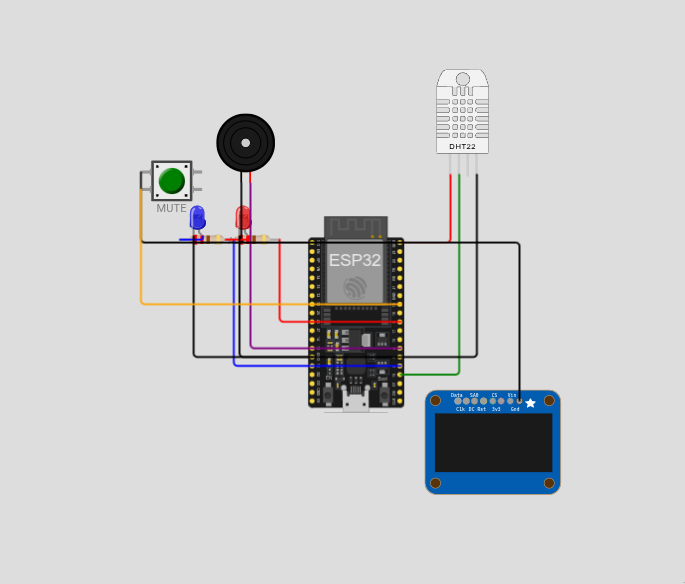
\includegraphics[width=10cm]{wokwi.png}
\end{center}

\vspace{1cm}

\subsection*{3. Pembagian Tugas Kelompok}
Dalam penyelesaian tugas pembuatan produk dan proposal ini, pembagian peran dalam kelompok kerja diatur sebagai berikut:
\begin{itemize}
    \item \textbf{Wisam Yassar Mahardika (Ketua Kelompok \& Programmer):}\\ Bertanggung jawab memimpin jalannya proyek, membuat baris kode program IoT, dan memastikan produk berfungsi dengan baik.
    \item \textbf{Devant Fadhillah (Teknisi Perangkat Keras):}\\ Bertugas merakit komponen mikrokontroler, menyolder kabel, dan memasang sensor pada boks pelindung.
    \item \textbf{Sandika Eka Permadi (Desainer Visual):}\\ Bertanggung jawab mendesain logo, merancang bentuk boks produk, serta mengatur tata letak antarmuka di layar HP.
    \item \textbf{Rafli Saeful Rukmana (Analis Jaringan):}\\ Bertugas merancang pengaturan WiFi, memastikan koneksi stabil, dan memikirkan letak penempatan alat yang pas di dalam rak server.
    \item \textbf{Aliif Abdu Mukti Al-Ghifari (Pemasaran \& Keuangan):}\\ Mencatat rincian pengeluaran modal, menghitung harga jual, dan menyusun isi bahasa proposal yang menarik.
\end{itemize}

\end{document}
